%!TEX root = thesis.tex

\chapter{Analyse}
\label{chapter-analyse}

Dieses Kapitel beschreibt alle für die Arbeit notwendigen Grundlagen.

\section{Datenquellen}
\label{section:daten}
Für die Analyse wurden Stakeholder-Interviews durchgeführt. Die Interviews fanden im Mai 2022
auf dem Universitätsgelände oder online statt. Die Befragten wurden durch ein qualitatives,
semi-strukturiertes Interview geführt. Im Vorfeld wurde dafür ein Interviewleitfaden entwickelt
(Anhang Verlinken). Es wurde eine Unterteilung in Verleihende und Ausleihende von Assets vorgenommen
(genaue Definition der Benutzergruppen in Abschnitt
\ref{section:benutzer}). Bei den Teilnehmenden handelt es sich um Mitarbeitende und Studierende der
Universität zu Lübeck, welche am \ac{imis} tätig sind. In \ref{table:e} sind die Rollen der befragten
Verleihenden aufgeführt. Die Verleihenden der Assets können gleichzeitig auch die Rolle der
Ausleihende einnehmen. Die Rollen der befragten Ausleihende sind in \ref{table:b} dargestellt. Die IDs
der Tabellen werden als Verweise in den folgenden Abschnitten verwendet.


\begin{table}[h]
    \centering
    \begin{zebratabular}{ll}
        \headerrow ID & Rolle \\
            V1 & Professor\\
            V2 & Wissenschaftlicher Mitarbeiter\\
            V3 & Wissenschaftlicher Mitarbeiter \\
            V4 & Sekretariat und administratives Personal\\
    \end{zebratabular}  
    \caption{Teilnehmende der Interviews, Verleihende}
    \label{table:e}
\end{table}

\begin{table}[h]
    \centering
    \begin{zebratabular}{ll}
        \headerrow ID & Rolle \\
            A1  & Bachelorstudent und Hilfswissenschaftler\\
            A2 & Bachelorstudent\\
            A3  & Masterstudent und Hilfswissenschaftlerin\\
    \end{zebratabular}
    \caption{Teilnehmende der Interviews, Ausleihende}
    \label{table:b}
    \hfill
    
\end{table}

\section{Benutzeranalyse}
\label{section:benutzer}

\section{Aufgabenanalyse}
\label{section:aufgaben}

\section{Kontextanalyse}
\label{section:kontext}

\section{Analyse des aktuellen Stands}
\label{section:iststand}

Snipe-IT ist eine kostenlose, quelloffene IT-Asset-Verwaltungs-Plattform,
welche das Nachverfolgen von Software-Lizenzen, Hardware und
Verbrauchsgegenständen ermöglicht. Genannte Assets können über ein Dashboard
hinzugefügt, verwaltet und gelöscht werden. Über Labels können Assets zur
Übersichtlichkeit in verschiedene Kategorien eingeordnet werden, während
Tags ein Asset eindeutig identifizieren (z. B. Seriennummer). Zudem ermöglicht
das „Checkin/Checkout“-System die Nachverfolgung aller Assets, falls diese
z. B.  an Person ausgeliehen werden. Zu jedem Zeitpunkt kann ein Asset
maximal einer Person zugeordnet werden, wodurch das mehrfache gleichzeitige
Ausleihen eines Assets verhindert wird. Darüber hinaus beschreiben Status-Label
den Zustands eines Assets und ob dieses ausgeliehen werden kann. Alle
Funktionalitäten können zudem über eine REST-API programmatisch genutzt werden.


\section{Formalisierte Anforderungen}
\label{section:anforderung}

Im Folgenden werden systematisch formalisierte Anforderungen präsentiert, welche die Ergebnisse der Analysen abschließend zusammenfassen.
Es werden zunächst die Visionen und Ziele (\ref{section:visionziel}) definiert, des Weiteren werden
die Rahmenbedingungen (\ref{section:rahmen}) und der Kontext des Systems
(\ref{section:kontextueberblick}) dargestellt. Darauf aufbauend wird eine funktionale Anforderung
erstellt (\ref{section:funktionale}). Abschließen werden die Qualitätsanforderungen formuliert
(\ref{section:qualität}).


\subsection*{Vision und Ziele}
\label{section:visionziel}
Zunächst sollten die Visionen und Ziele des Systems konkretisiert werden, an denen sich die
Anforderungen auf Zielgerichtetheit überprüfen lassen \cite{balzert2009}. Diese setzen sich aus der
Analyse der Benutzenden sowie Aufgaben und des Kontextes zusammen. Im ersten Schritt werden die
Visionen für die Zukunft realitätsnah festgelegt.



\begin{center}
        \renewcommand{\arraystretch}{1.5}
        \begin{tabular}{p{0.1\textwidth}p{0.8\textwidth}}
                \hline
                \textbf{/V10/} & Verleihende des Status sind in der Lage,                                          \\
                \textbf{/V20/} & Ausleihende sind besser dazu in der Lage,                                         \\
                \hline
        \end{tabular}
\end{center}

Basierend auf diese Visionen lassen sich die Ziele formulieren, welche die Visionen
operationalisieren. Diese folgen dabei den standardisierten Regeln zur Formulierung von Zielen
\cite{pohl_requirements_2008}.


\begin{center}
        \renewcommand{\arraystretch}{1.5}
        \begin{tabular}{p{0.1\textwidth}p{0.8\textwidth}}
                \hline
                \textbf{/Z10/} & Ausleihende eines Assets erhalten zielgerichtete und aktuelle
                Informationen zum Verbleib der.                                                                          \\
                \textbf{/Z20/} & XX sind jederzeit in der Lage, ihre Informationen zu ändern.                                       \\
                \textbf{/Z40/} & XX sind überall in der Lage, ihre Informationen zu ändern.                                         \\
                \textbf{/Z50/} & Der Status ist durch XX leicht und unkompliziert veränderbar.                                      \\
                \hline
        \end{tabular}
\end{center}

\subsection*{Rahmenbedingungen}
\label{section:rahmen}
Die Randbedingungen legen organisatorische und technische Restriktionen für das System oder den
Entwicklungsprozess fest \cite{balzert2009}. Die Bedingungen wurden aus dem Lastenheft und der
Benutzer- und Kontextanalyse abgeleitet.

\begin{center}
        \renewcommand{\arraystretch}{1.5}
        \begin{tabular}{p{0.1\textwidth}p{0.8\textwidth}}
                \hline
                \textbf{/R10/} & Das System ist eine Web-Anwendung.                                                        \\
                \textbf{/R20/} & Die Zielgruppe sind Mitarbeitende des IMIS und Studierende.                               \\
                \textbf{/R30/} & Die Zielgruppe teilt sich in zwei Nutzergruppen: die Verleihenden und
                Ausleihende von Assets. Die Definitionen der Nutzergruppen sind in Kapitel (\secref{section:benutzer})
                zu finden.                                                                                                 \\
                \textbf{/R40/} & Das System wird von Verleihenden sowohl im mobilen als auch im Arbeitskontext genutzt (). \\
                \textbf{/R50/} & Die eingesetzte Software auf der Zielmaschine ist clientseitig ein
                Webbrowser. Die marktführenden Webbrowser müssen unterstützt werden: Chrome, Firefox,
                Safari \cite{noauthor_browser_nodate}.                                                                     \\
                \hline
        \end{tabular}
\end{center}

\subsection*{Kontext und Überblick}
\label{section:kontextueberblick}
Ein System ist in einer technischen Umgebung eingebettet \cite{balzert2009}. Es wurde im Folgenden Bezug auf das aktuelle Vorgehen und die Schnittstellen des System genommen.

\begin{center}
        \renewcommand{\arraystretch}{1.5}
        \begin{tabular}{p{0.1\textwidth}p{0.8\textwidth}}
                \hline
                \textbf{/K10/} & Das aktuelle Vorgehen umfasst Klebezettel an den Türen der Mitarbeitenden.                                                                  \\
                \textbf{/K20/} & Es existiert eine Schnittstelle zum Back-End des Labormanagementsystems.                                                                    \\
                \textbf{/K30/} & Es existiert ein digitaler Kalender, auf den die Mitarbeitenden Zugriff haben, in dem geblockte Zeiten einzelner Personen angezeigt werden. \\
                \hline
        \end{tabular}
\end{center}

\subsection*{Funktionale Anforderungen}
\label{section:funktionale}
Im Folgenden werden die Kernfunktionalitäten des Systems aufgeführt \cite{balzert2009}.
Diese ergeben sich aus der Aufgabenanalyse (\ref{section:aufgaben}). Um die Anforderungen mit einer eindeutigen Semantik zu formulieren, wurde eine Anforderungsschablone (\ref{fig:schablone}) verwendet, um natürlichsprachliche Anforderungen zu definieren \cite{balzert2009}.

\begin{figure}[h]
        \centering
        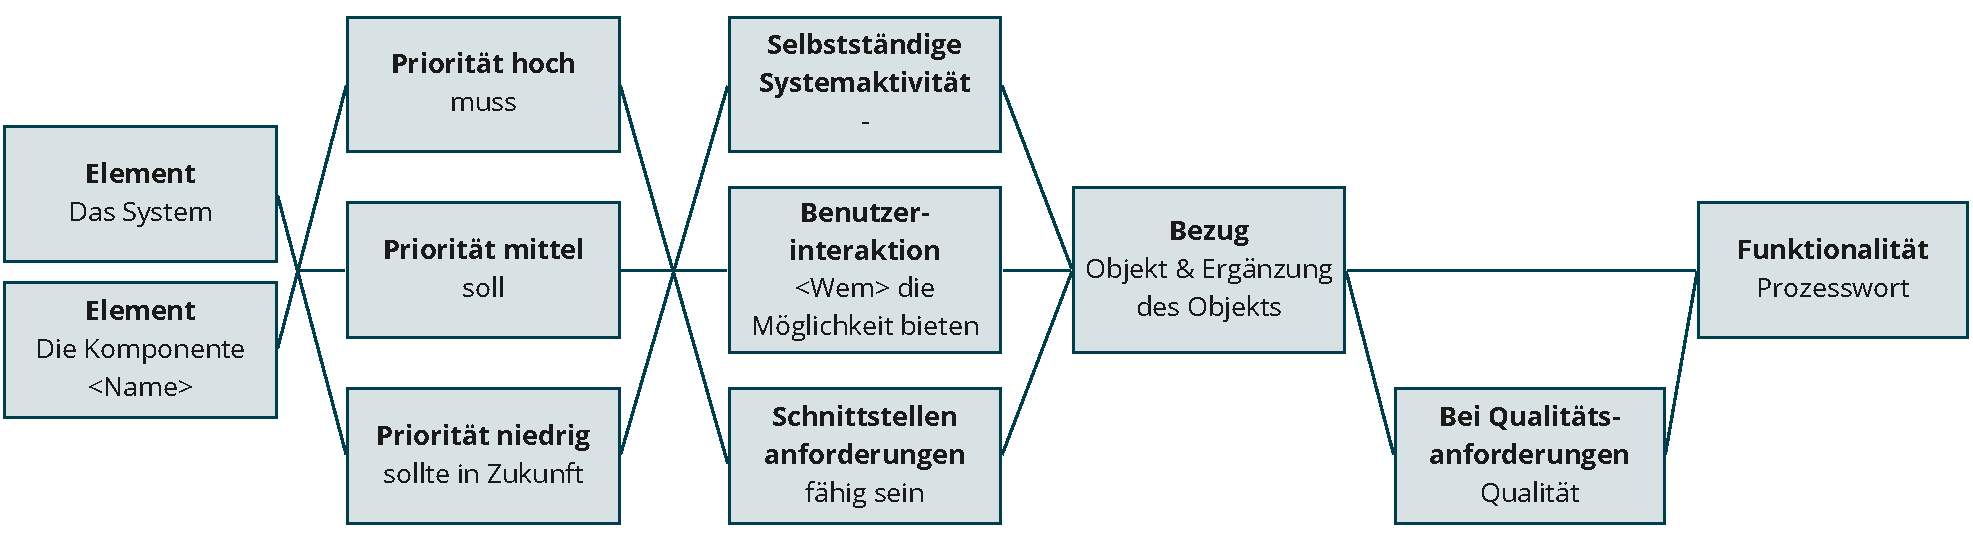
\includegraphics[scale=0.45]{Bilder/anforderungsschablone.pdf}
        \label{fig:schablone}
        \caption[Anforderungsschablone]{Anforderungsschablone \cite{balzert2009}}
\end{figure}

\begin{center}
        \renewcommand{\arraystretch}{1.5}
        \begin{tabular}{p{0.1\textwidth}p{0.8\textwidth}}
                \hline
                \textbf{/F10/}  & Das System \textit{muss} XX die Möglichkeit bieten, Informationen jederzeit einzutragen (A).                             \\
                \textbf{/F20/}  & Das System \textit{muss} XX die Möglichkeit bieten, Status wiederzuverwenden.                                            \\
                \textbf{/F30/}  & Das System \textit{muss} XX die Möglichkeit bieten, ein Profil zu erstellen (A).                                         \\
                \textbf{/F40/}  & Das System \textit{muss} XXn relevante Informationen anzeigen, welche vom Erstellenden hinterlassen werden sollen (A).   \\
                \textbf{/F50/}  & Das System \textit{muss} XX die Möglichkeit geben, den alleinigen Zugriff auf die eigenen Daten zu haben.                \\
                \textbf{/F60/}  & Das System \textit{soll} XX die Möglichkeit bieten, individuelle und personalisierte Inhalte zu visualisieren (A).       \\
                \textbf{/F70/}  & Das System \textit{soll} daran erinnern, die Informationen zu aktualisieren (A).                                                   \\
                \textbf{/F80/}  & Das System \textit{soll} XX die Möglichkeit bieten, sich eine Vorschau ihres aktuell angezeigten Türschilds anzuschauen. \\
                \textbf{/F90/}  & Das System \textit{sollte in Zukunft} XX.                                     \\
                \textbf{/F100/} & Das System \textit{sollte in Zukunft} XX die Möglichkeit bieten, Informationen zu hinterlassen (A).                     \\
                \textbf{/F110/} & Das System \textit{sollte in Zukunft} den angezeigten Status automatisch aus den Daten des digitalen Kalenders ermitteln können.   \\
                \hline
        \end{tabular}
\end{center}


\subsection*{Qualitätsanforderungen}
\label{section:qualität}
Im letzten Schritt werden die nicht-funktionalen Anforderungen festgelegt, welche die qualitativen oder quantitativen Eigenschaften eines Systems darstellen \cite{balzert2009}. Auch hier wird, falls möglich, die Anforderungsschablone aus \ref{fig:schablone} verwendet.

\begin{center}
        \renewcommand{\arraystretch}{1.5}
        \begin{tabular}{p{0.1\textwidth}p{0.8\textwidth}}
                \hline
                \textbf{/Q10/} & Das System \textit{muss} den Grundsätzen der DIN EN ISO
                9241-110:2019-09 (Ergonomie der Mensch-System-Interaktion - Teil 110:
                Interaktionsprinzipien) folgen (\textit{DIN EN ISO 9241-110}, 2019).                                                                                                                \\
                \textbf{/Q20/} & Das System \textit{muss} die definierten Nutzungsklassen aus Kapitel
                section:benutzer (Sonderrolle) unterscheiden und die dazugehörigen Zugriffsrechte
                sicherstellen.                                                                                                                                                                      \\
                \textbf{/Q30/} & Das System \textit{soll} modular strukturiert sein, damit Inhalte und Funktionalitäten effizient eingebunden werden können und das System einfach erweiterbar ist. \\
                \textbf{/Q40/} & Das System \textit{soll} beim Zugriff über das Internet eine gesicherte Übertragung (bspw. \ac{HTTPS}) ermöglichen.                                                     \\
                \textbf{/Q50/} & Das System \textit{soll} alle Benutzerinteraktionen in unter fünf Sekunden ausführen.                                                                              \\
                \hline
        \end{tabular}
\end{center}
